\documentclass{report}
\usepackage[utf8]{inputenc}
\usepackage{hyperref}
\usepackage{amsmath}
\usepackage{bera}
\usepackage{listings}
\usepackage{xcolor}
\usepackage{graphicx}

\graphicspath{{../../figures/}}

\title{
    {Moral AI IQP}\\
    {\large Worcester Polytechnic Institute}\\
    {
\includegraphics[height=2in]{figures/WPI_Inst_Prim_FulClr.png}}
}
\author{Ryan Benasutti}
\date{March 2019}

\newcommand{\code}{\texttt}

\begin{document}

\maketitle

\clearpage
\mbox{}
\clearpage

\chapter*{Abstract}

Artificial intelligence is being deployed in increasingly autonomous systems where it will have to
make moral decisions. However, the rapid growth in artificial intelligence is outpacing the research
in building explainable systems. In this paper, a number of problems around one facet of explainable
artificial intelligence, training data, are explored. A solution to these problems is presented.
Additionally, the human decision making process in unavoidable accident scenarios is explored.

\chapter*{Acknowledgements}

\begin{enumerate}
    \item Professor Therese Smith
    \item Professor Yunus Telliel
    \item Griffin Tabor
\end{enumerate}

\tableofcontents

\chapter{Introduction}

\begin{enumerate}
    \item Autonomous vehicle technology is growing rapidly and AI is a key piece of that technology.
    As this technology gets closer to attaining full autonomy, the AI deployed in these systems will
    have greater responsibility than ever. These AI systems must be explainably fair, i.e. they must
    both make decisions using only the least amount of information necessary for optimal performance
    and make those decisions predictably and correctly. For example, the AI in an autonomous vehicle
    does not need to be supplied with information about a pedestrian's race, even though race may be
    an impactful trait in other fields, especially medical fields \cite{sickeCellDisease}.
    Furthermore, these AI systems must also be explainable for legal reasons, such as determining
    which party is at fault in the event of a car accident or, in the European Union, complying with
    a user's "right to explanation" \cite{goodman2017european}.
    
    \item The demand for explainable AI is increasing, such as DARPA's Explainable Artificial
    Intelligence (XAI) program \cite{gunning2016explainable}. This program aims to develop
    explainable AI systems such as in Figure~\ref{fig:darpa_xai}. There has also been a symposium
    focusing on AI inclusivity towards marginalized peoples \cite{berkmanKleinCenterAI2017}
    \cite{aiAndInclusionSymposium}. This symposium illustrates the increasing need to discuss AI
    fairness and inclusivity in a way that non-technical people can understand. One facet of this
    need that this paper addresses is the question of specifically how much one needs to care about
    possible biases in the various stages of AI architecture.
    
    \item We seek to demonstrate how an AI can learn a bias and empirically determine the severity
    of that bias. Classification accuracy testing will be employed to evaluate the trained AI and
    determine if any bias was learned, and, if so, the severity of that bias.

    \item We also seek to understand the decision making process in humans behind making moral
    decisions in unavoidable accident scenarios, i.e. dilemmas. This part of the research will be
    done by surveying a group of people and performing qualitative analysis on the survey results.
\end{enumerate}

\chapter{Background}

\begin{enumerate}
    \item Introduce background readings.
    
    \item Cite examples of AI that must (or will in the near future) make moral decisions.
    \begin{itemize}
        \item \cite{bojarski2016end} performs end-to-end learning which "map raw pixels from a
        single front-facing camera directly to steering commands". With this approach, the AI will
        have to directly respond to pedestrians and other external stimuli.
    \end{itemize}
    
    \item The Moral Machine experiment \cite{awad2018moral} is prior research into people's
    preferences in moral dilemmas. Participants are shown a moral dilemma involving an autonomous
    vehicle, passengers, and pedestrians. In each dilemma, the participant must choose between
    inaction, which results in the certain death of the pedestrians, and action, which results in
    certain death of the passengers. The study revealed three strong global preferences towards
    sparing humans over animals, sparing more lives rather than fewer, and sparing younger lives
    rather than older. The study also showed that some preferences vary between countries depending
    on that country's propensity towards egalitarianism.
\end{enumerate}

\chapter{Methods}

\section{Data Generation}

The data is generated using a graphical model to control the conditional probabilities for the
states of each variable. The variables in the model correspond directly to the attributes of a
person. Figure~\ref{fig:graphical_model_image} is a rendering of the graphical model. For example,
people in the first option could be more likely to jaywalk then people in the second option,
producing a data set which is biased towards/against jaywalkers. When combined with control over the
number of people in each option, this method can produce both subtle and strong bias. The code for
the domain of each attribute of a person is in Figure~\ref{fig:code_for_person_attribute_domains}.
\href{https://github.com/pgmpy/pgmpy}{pgmpy} is used to create the graphical model and infer each
variable’s probability distribution. These distributions are then used to pick elements from each
variable’s domain. This process is repeated for each attribute of each person and for the num- ber
of people in each option of a dilemma, forming a complete dilemma. The number of dilemmas generated
is specified programmatically using the \code{TrainMetadata} class, which captures the number of
dilemmas to generate and the maximum number of people per option.

\begin{figure}
    \centering
    \begin{verbatim}
    age_states = [10, 20, 30, 40, 50, 60]
    race_states = [Race.white, Race.black, Race.asian,
                Race.native_american, Race.other_race]
    legal_sex_states = [LegalSex.male, LegalSex.female]
    jaywalking_states = [False, True]
    driving_under_the_influence_states = [False, True]
    \end{verbatim}
    \caption{Python code for the bracketed attributes of a Person}
    \label{fig:code_for_person_attribute_domains}
\end{figure}

\section{Data Bracketing}

Attributes are one-hot encoded so the neural network is resilient to unspecified attributes. Age is
bracketed by increments of 10 years. Some example encoded ages are shown in
Table~\ref{tab:example_age_attribute_encoding}. Boolean attributes are encoded into three
increments, as shown in Table~\ref{tab:example_boolean_attribute_encoding}.
    
\begin{table}
    \centering
    \begin{tabular}{c|c|c|c|c|c|c|c}
        Age (yr) & unspecified & 1-10 & 11-20 & 21-30 & 31-40 & 41-50 & 51-60 \\\hline
        unspecified & 1 & 0 & 0 & 0 & 0 & 0 & 0 \\
        0 & 0 & 1 & 0 & 0 & 0 & 0 & 0 \\
        3 & 0 & 1 & 0 & 0 & 0 & 0 & 0 \\
        16 & 0 & 0 & 1 & 0 & 0 & 0 & 0 \\
        42 & 0 & 0 & 0 & 0 & 0 & 1 & 0
    \end{tabular}
    \caption{Example age attribute encoding.}
    \label{tab:example_age_attribute_encoding}
\end{table}

\begin{table}
    \centering
    \begin{tabular}{c|c|c|c}
        Value & unspecified & false & true \\\hline
        unspecified & 1 & 0 & 0 \\
        false & 0 & 1 & 0 \\
        true & 0 & 0 & 1
    \end{tabular}
    \caption{Example boolean attribute encoding.}
    \label{tab:example_boolean_attribute_encoding}
\end{table}

\section{Data Storage}

Data is stored using the JSON format using a serialization process called pickling via the Python
library \href{https://jsonpickle.github.io/}{jsonpickle}. This process was chosen because it
produces easily machine-readable files and because JSON is a popular data storage format. The
purpose of storing the generated data sets is to keep the data consistent between test iterations
and to share the data. Both the training and test data sets are pickled after generation.

\section{Neural Network Model}

There are two primary requirements of the neural network used in the experiments. First, the network
must classify the training data. In other words, when given a dilemma, the network must classify
that dilemma based on which option is most preferable. For example, in a dilemma with two options of
three and four people, respectively, the correct classification is the second option because it has
more people. In the case where a dilemma has two or more options of equal size, the earlier option
is chosen.

Second, the network must be easy to train, meaning that the time required to train the network must
be small (on the order of minutes or less) and the hardware resources required to train the network
must be minor. Testing the network requires training it many times, so the time required to train
the network must be small. Additionally, the network will be trained on personal machines, so any
hardware requirements must be easy to meet.

The final neural network chosen is a simple, shallow, feed-forward network with one hidden layer
trained using supervised learning \ref{fig:shallow_neural_network}. There are three alternative
models which were considered. First, an autoencoder. Autoencoders are trained using unsupervised
learning, so labeling the data is not necessary (want to avoid imparting a set of morals). This
model would perform dimensionality reduction, and perhaps learn to ignore noise (i.e. uniformly
distributed attributes) in the data set, but would be unable to classify the dilemmas.

Second, an autoencoder in combination with a simple neural network trained using supervised
learning. This model solves the classification problem which the previous model failed at, but
introduced unnecessary complexity to the research. The intent of this research is not to build a
neural network capable of guiding a real autonomous vehicle.
    
Lastly, a recurrent neural network (RNN) with long short-term memory (LSTM). This option was
considered because RNN's are capable of accepting variable-length sequential data; however, this
network does not solve the classification problem, so it is unusable for this research.

\section{Neural Network Training}

The neural network is modeled and trained using Keras. The input layer has dimensionality equal to
the number of attributes per person (after one-hot encoding) multiplied by the number of options per
dilemma multiplied by the maximum number of people per option. The output layer has dimensionality
equal to the number of options per dilemma. The hidden layer has dimensionality equal to the average
of that of the input and output layers. An example implementation in Keras can be seen in
Figure~\ref{fig:code_for_keras_model}; additionally, Figure~\ref{fig:neural_network_model} provides
a simple visualization of the dimensionality of the network.

\begin{figure}
    \centering
    \begin{verbatim}
    output_dim = 2
    input_dim = 22 * output_dim * \
            train_metadata.max_num_people_per_option

    model.add(Dense(units=input_dim, activation='relu',
                input_dim=input_dim))
    model.add(Dense(units=round((input_dim + output_dim) / 2),
                activation='relu'))
    model.add(Dense(units=output_dim, activation='softmax'))
    \end{verbatim}
    \caption{The Keras code for the neural network model.}
    \label{fig:code_for_keras_model}
\end{figure}

\section{Neural Network Testing}

The neural network is tested using Keras to evaluate the classification accuracy and loss against a
test data set. The test data is generated in the same way as the training data, though typically
with less or no bias. Each training data set is tested five times. Each iteration involves training
the neural network on the training data set and evaluating its performance against a test data set
to collect classification accuracy and loss information. The results of all five runs are averaged
to produce an average classification accuracy and loss.

\chapter{Findings and Analysis}

\section{Response to Bias}

Our research found that the AI became biased when the training data featured a strong trend not
present in the test data. For purposes of a control test, a test data set was generated with
uniformly distributed people and a uniformly distributed jaywalking probability.
Figure~\ref{fig:test_50-50_50-50_50-50_accuracy_plot} shows the result of this test. In this
scenario, $P(J)$ is observed to be independent of $P(O_1)$. When $P(J \mid O_1) < 0.1$, the neural
network classifies dilemmas incorrectly. This trend continues as $P(J \mid O_1)$ decreases, thereby
increasing the severity of the bias in the training data set. A similar but opposite trend occurs
when $P(J \mid O_1) > 0.9$.

Observing the contour plot in Figure~\ref{fig:test_40-60_100-0_0-100_accuracy_plot}, one can see
that classification accuracy decreases abnormally (i.e. differently than in the control in
Figure~\ref{fig:test_50-50_50-50_50-50_accuracy_plot}) when $P(O_1) > 0.6$ and $P(J \mid O_1) <
0.2$. In this area, the training data set consists mostly of people in the first option. Most people
in the first option are not jaywalkers and most people in the second option are. Therefore, the
training data set is biased to prefer non-jaywalkers because they appear disproportionately
frequently in the (larger) first option. The neural network, now having learned this trend, is
tested against a test data set in which most people are in the second option. Those in the first
option are not jaywalkers and those in the second option are. The network tends to select the first
option because it contains far fewer jaywalkers than the second option, despite the first option
being smaller than the second and therefore the incorrect choice. This causes the network's
classification accuracy to decrease in this region. The trend continues as $P(O_1)$ increases while
$P(J \mid O_1)$ decreases, thereby increasing the severity of the bias in the training data set.
Another view into the network's decisions is Figure~\ref{fig:test_40-60_100-0_0-100_jay_prob_plot},
which shows the real value of $P(J)$ when the network classified a dilemma incorrectly. In the areas
of the contour plot corresponding to Figure~\ref{fig:test_40-60_100-0_0-100_accuracy_plot}'s areas
of worst accuracy, we can see that the real value of $P(J)$ is close to zero. In other words, the
network performs worst when it picks an option because that option is absent of jaywalkers (i.e.
when the network makes a decision based on the bias it learned rather than the rule used to label
the test data set). This is further evidence that the network has learned a bias against jaywalkers.
A similar but opposite trend occurs when $P(O_1) < 0.4$ and $P(J \mid O_1) > 0.8$.

\section{Avoiding Bias}

Three ways for the neural network to learn a bias
\begin{enumerate}
    \item Flaws in data
    \begin{enumerate}
        \item Any information which is not strictly necessary for the neural network to make
        effective decisions should not be given to the network.

        \item Neural networks used for object detection in images suffer from predictive inequality
        in detecting people of differing skin tones \cite{wilson2019predictive}. Those with skin
        tones in the Fitzpatrick range $[1-3]$ are more accurately identified than those with skin
        tones in the $[4-6]$ range. Furthermore, this problem persists between networks of different
        architectures. Although the authors of that research propose a different loss function which
        decreases predictive inequality, one could imagine a totally different architecture which
        does not use color cameras at all; namely, infrared cameras can not suffer from this class
        of problem.
    \end{enumerate}
    
    \item Flaws in AI architecture
    \begin{enumerate}
        \item This research uses a simple, shallow neural network to reduce architectural
        complexity. Deeper networks, specifically deep convolutional networks, undoubtedly perform
        better, but these network architectures suffer from increased design complexity and
        increased training difficulty \cite{mhaskar2016deep}.
    \end{enumerate}
    
    \item Flaws in testing
    \begin{enumerate}
        \item If one is concerned that a system may be less able to measure some attribute in a
        certain environment, then the testing for the system may want to overrepresent that
        attribute.

        \item If a system should be equally sensitive to all of its inputs, then those input should
        be represented equally during testing, even if a different distribution of inputs is
        expected to be encountered when the system is deployed. In the case of autonomous vehicles,
        this research assumed the neural network should treat all people equally, but in reality
        this is a region-specific measure. The Moral Machine experiment measured strong regional
        preferences for various aspects of decision-making during unavoidable accident scenarios
        \cite{awad2018moral}. For example, Eastern countries showed an almost nonexistent preference
        for sparing the young compared to Western and Southern countries. Southern countries showed
        a strong preference for sparing females compared to Western and Eastern countries. Not all
        regional preferences can be reliably accounted for, however. Some preferences, such as the
        Eastern countries stronger preference for sparing the lawful compared to Western and
        Southern countries, is not entirely enforceable by AI systems. Some instances of lawfulness
        classification could be reliable, such as detecting jaywalkers, but others, such as
        detecting unlawful intoxication, are most likely difficult. There is, of course, the
        question of whether or not autonomous vehicles should contain any regional preferences or
        whether they should be totally fair; however, that is outside the scope of this paper.
    \end{enumerate}
\end{enumerate}
    
\section{Survey Results}

The survey results were ... and we extrapolate that the thought process behind these moral decisions
is ...

\chapter{Conclusion}

\begin{enumerate}
    \item Our research found that AI becomes biased when ?. Therefore, one must take a certain
    amount of care in dealing with bias in data (how much?).
    
    \item In order to avoid training biased AI, we recommend formatting training data such that ?.
    
    \item We also recommend that
    \begin{itemize}
        \item Teams that work with AI, especially teams which create or train AI, should include
        social scientists.
        
        \item AI could be verified by 3rd party groups in addition to a team's internal testing.
    \end{itemize}

    \item Future work includes
    \begin{itemize}
        \item Explanations, whether of AI decisions, architecture, or other, must be delivered in a
        way that the user can understand. As Gilpin puts it, "The success of this goal is tied to
        the cognition, knowledge and biases of the user: for a system to be interpretable, it must
        produce descriptions that are simple enough for a person to understand using a vocabulary
        that is meaningful to the user" \cite{gilpin2018explaining}. This paper has attempted to
        show specifically how much care one must take in dealing with bias in data, but more
        attention is needed in other areas of AI architecture.
    \end{itemize}
\end{enumerate}

\bibliography{citations}
\bibliographystyle{plain}

\appendix
\chapter{Figures}

\begin{figure}[h]
    \centering
    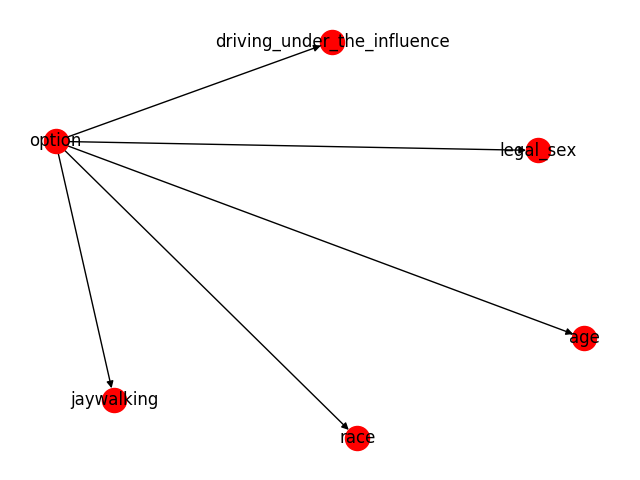
\includegraphics[scale=0.6]{figures/network.png}
    \caption[]{The graphical model.}
    \label{fig:graphical_model_image}
\end{figure}

\begin{figure}[h]
    \centering
    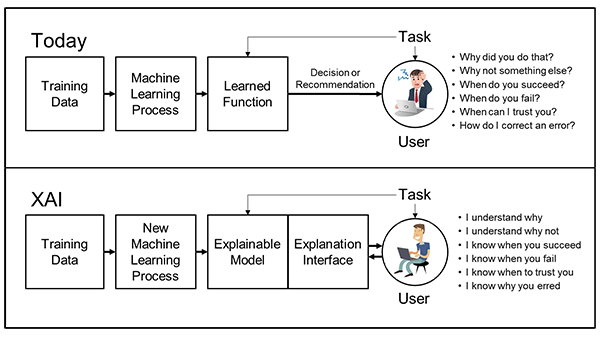
\includegraphics[scale=1.1]{figures/xai-figure2.png}
    \caption[]{DARPA's XAI Concept~\protect\cite{gunningXAIProgram}}
    \label{fig:darpa_xai}
\end{figure}

\begin{figure}[h]
    \centering
    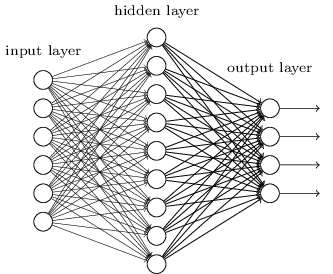
\includegraphics[scale=0.6]{figures/shallow_neural_network.png}
    \caption[]{A shallow feed-forward neural network with one hidden layer.}
    \label{fig:shallow_neural_network}
\end{figure}

\begin{figure}[h]
    \centering
    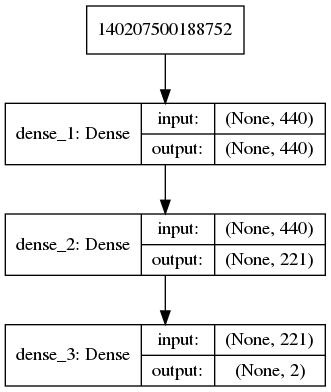
\includegraphics[scale=0.5]{figures/neural_network_model.png}
    \caption[]{The dimensions of the neural network used in this research.}
    \label{fig:neural_network_model}
\end{figure}

% 
% test 40-60 100-0 0-100
% 

\begin{figure}[h]
    \centering
    \centerline{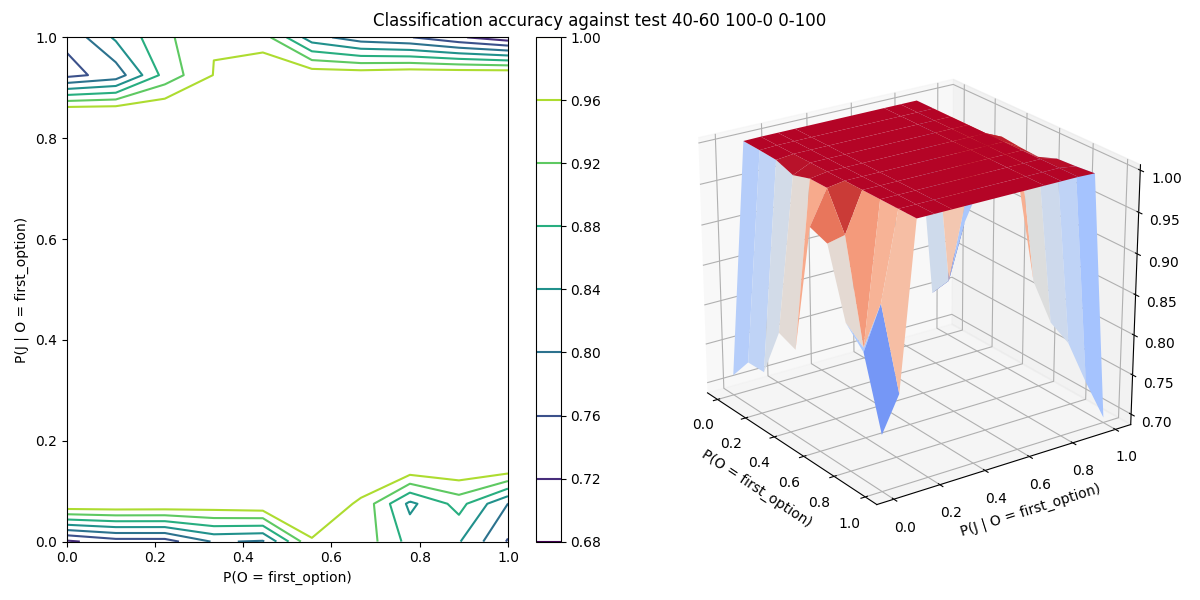
\includegraphics[scale=0.55]{test_40-60_100-0_0-100_accuracy.png}}
    \caption[]{The classification accuracy against \code{test 40-60 100-0 0-100}.}
    \label{fig:test_40-60_100-0_0-100_accuracy_plot}
\end{figure}

\begin{figure}[h]
    \centering
    \centerline{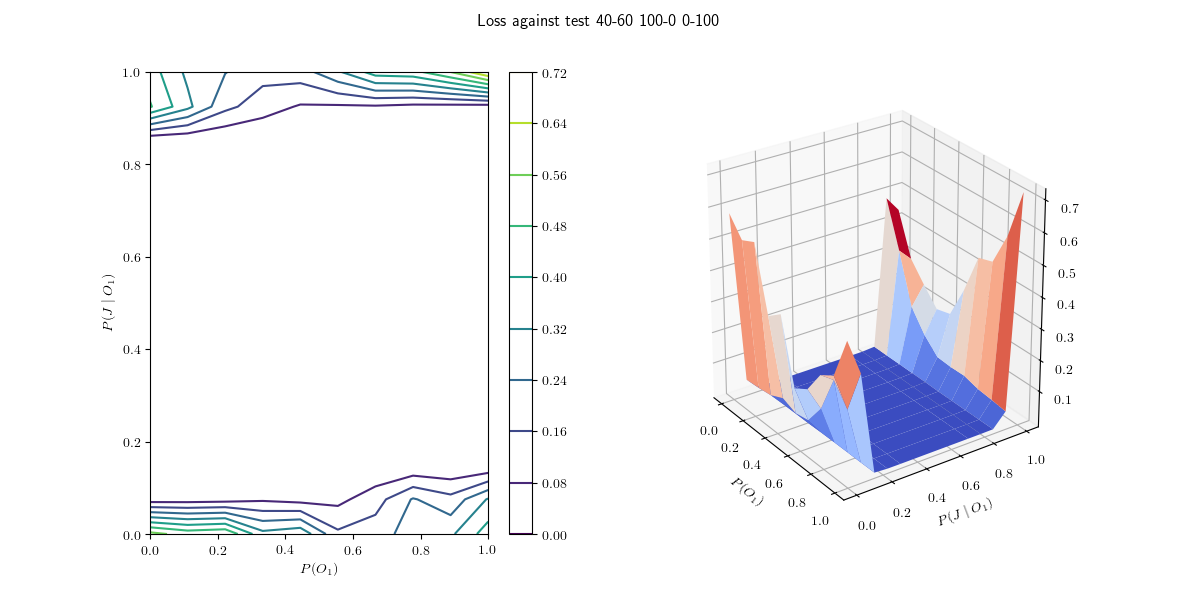
\includegraphics[scale=0.55]{test_40-60_100-0_0-100_loss.png}}
    \caption[]{The loss against \code{test 40-60 100-0 0-100}.}
    \label{fig:test_40-60_100-0_0-100_loss_plot}
\end{figure}

\begin{figure}[h]
    \centering
    \centerline{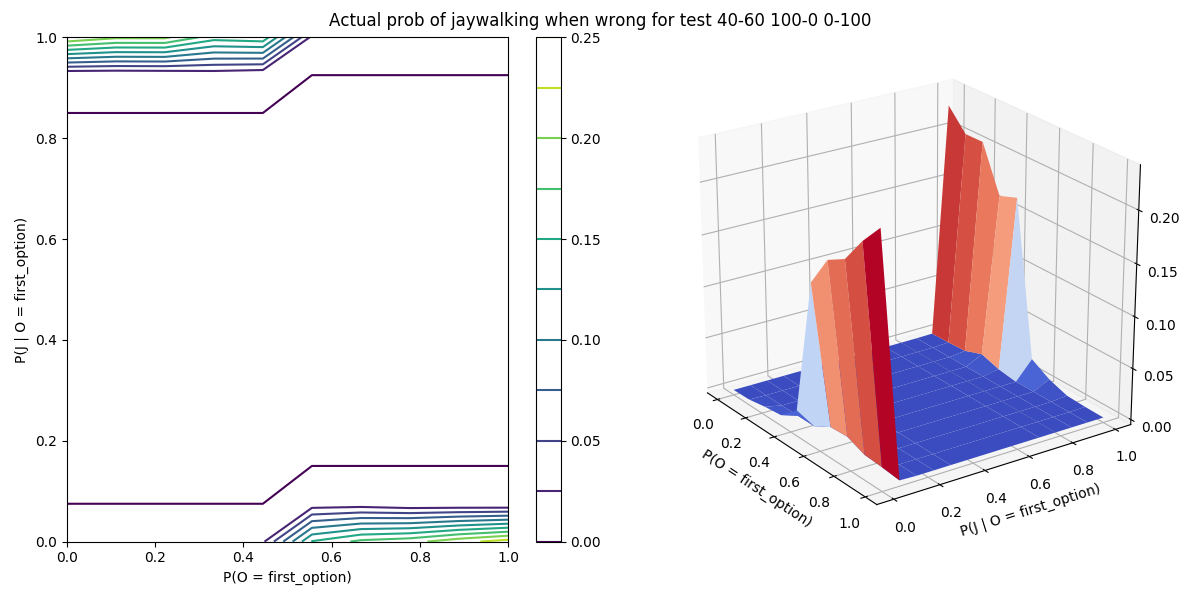
\includegraphics[scale=0.55]{test_40-60_100-0_0-100_jay_prob.png}}
    \caption[]{The actual jaywalking probability when classified incorrectly against \code{test 40-60 100-0 0-100}.}
    \label{fig:test_40-60_100-0_0-100_jay_prob_plot}
\end{figure}

% 
% test 40-60 0-100 100-0
% 

\begin{figure}[h]
    \centering
    \centerline{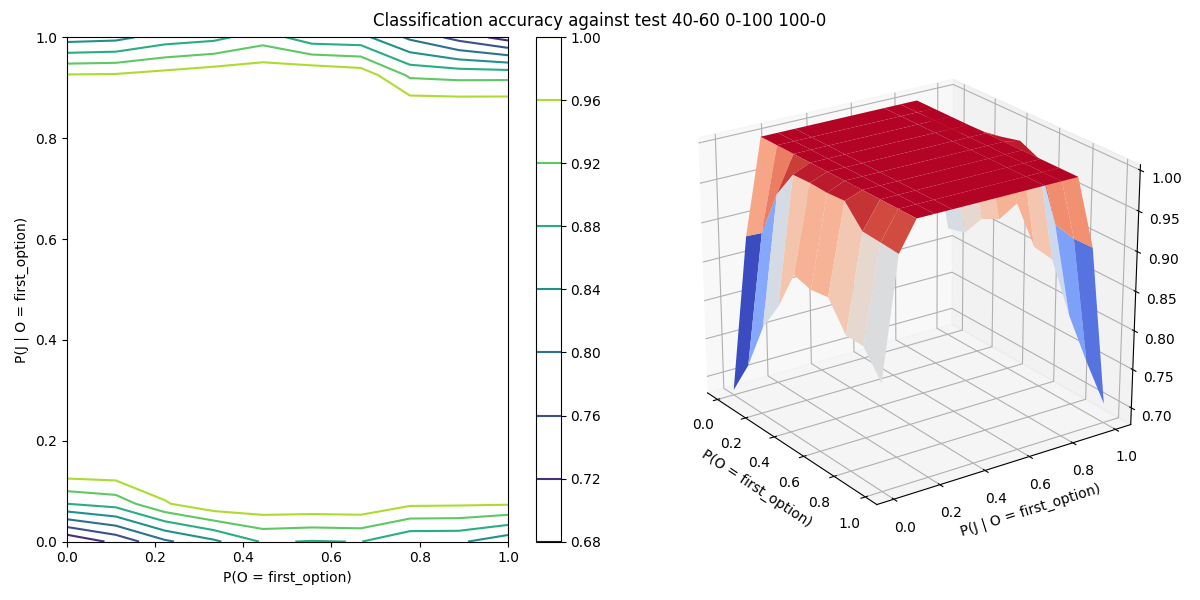
\includegraphics[scale=0.55]{test_40-60_0-100_100-0_accuracy.png}}
    \caption[]{The classification accuracy against \code{test 40-60 0-100 100-0}.}
    \label{fig:test_40-60_0-100_100-0_accuracy_plot}
\end{figure}

\begin{figure}[h]
    \centering
    \centerline{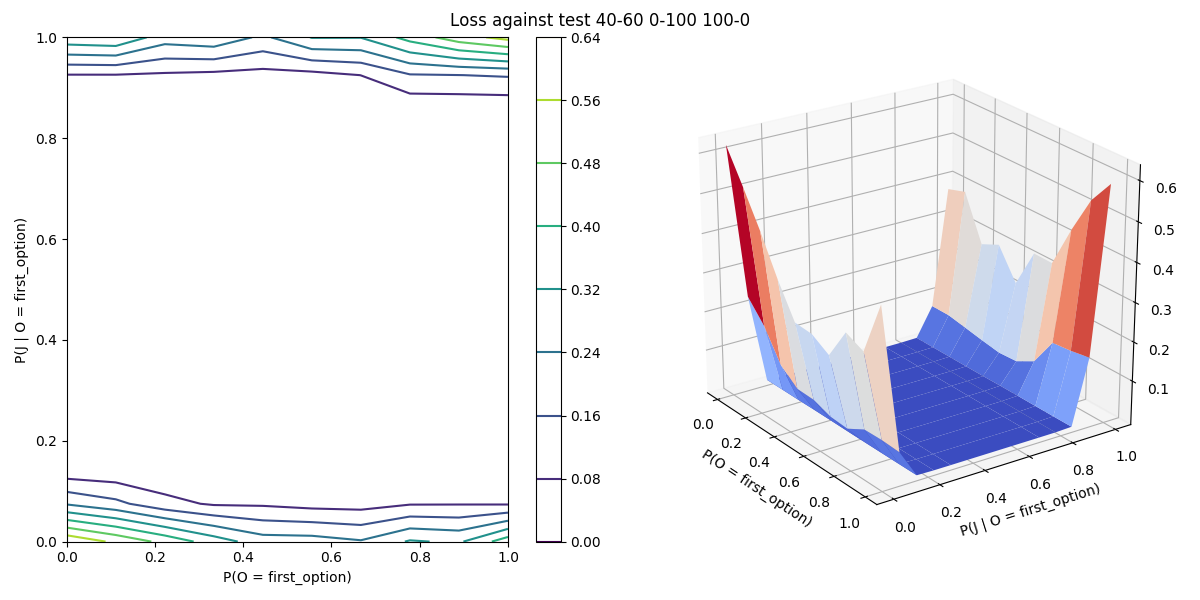
\includegraphics[scale=0.55]{test_40-60_0-100_100-0_loss.png}}
    \caption[]{The loss against \code{test 40-60 0-100 100-0}.}
    \label{fig:test_40-60_0-100_100-0_loss_plot}
\end{figure}

\begin{figure}[h]
    \centering
    \centerline{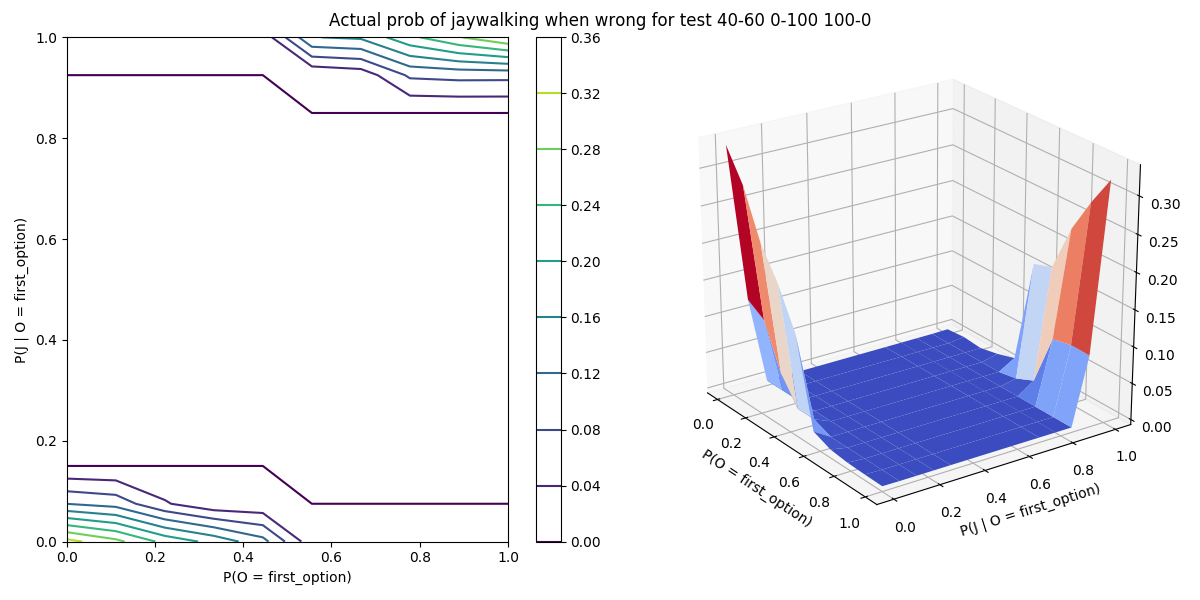
\includegraphics[scale=0.55]{test_40-60_0-100_100-0_jay_prob.png}}
    \caption[]{The actual jaywalking probability when classified incorrectly against \code{test 40-60 0-100 100-0}.}
    \label{fig:test_40-60_0-100_100-0_jay_prob_plot}
\end{figure}

% 
% test 40-60 80-20 20-80
% 

\begin{figure}[h]
    \centering
    \centerline{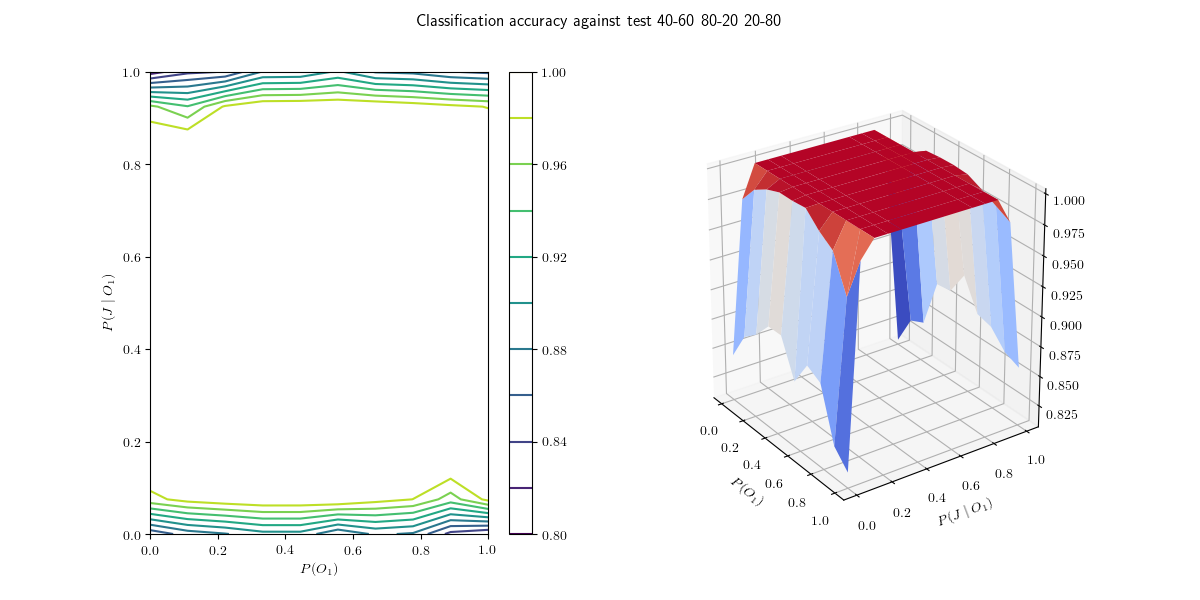
\includegraphics[scale=0.55]{test_40-60_80-20_20-80_accuracy.png}}
    \caption[]{The classification accuracy against \code{test 40-60 80-20 20-80}.}
    \label{fig:test_40-60_80-20_20-80_accuracy_plot}
\end{figure}

\begin{figure}[h]
    \centering
    \centerline{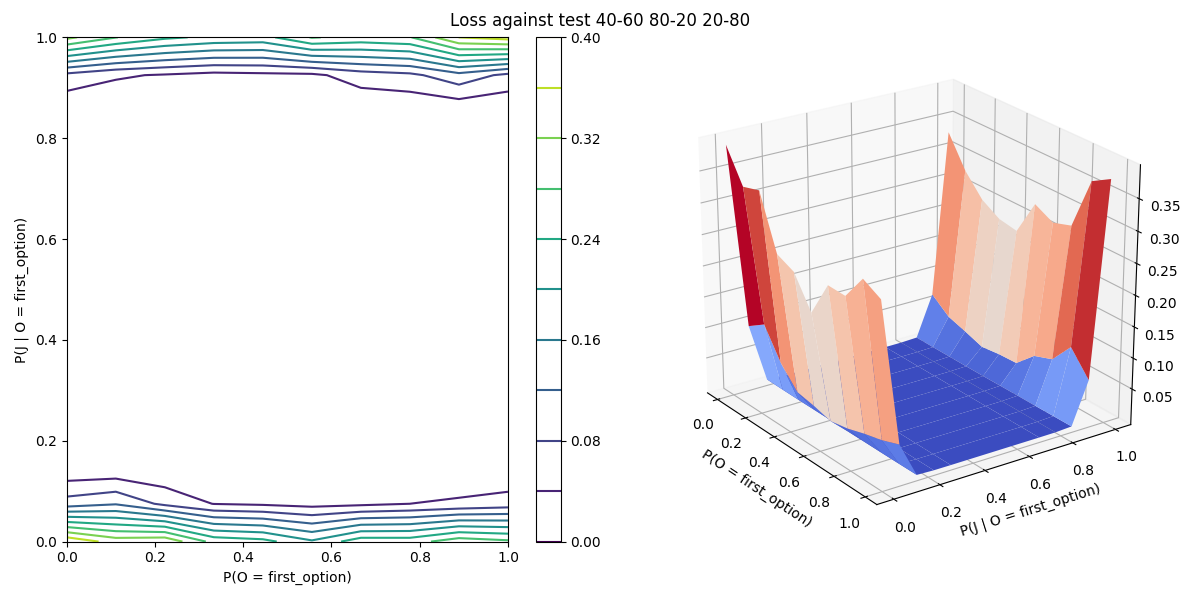
\includegraphics[scale=0.55]{test_40-60_80-20_20-80_loss.png}}
    \caption[]{The loss against \code{test 40-60 80-20 20-80}.}
    \label{fig:test_40-60_80-20_20-80_loss_plot}
\end{figure}

\begin{figure}[h]
    \centering
    \centerline{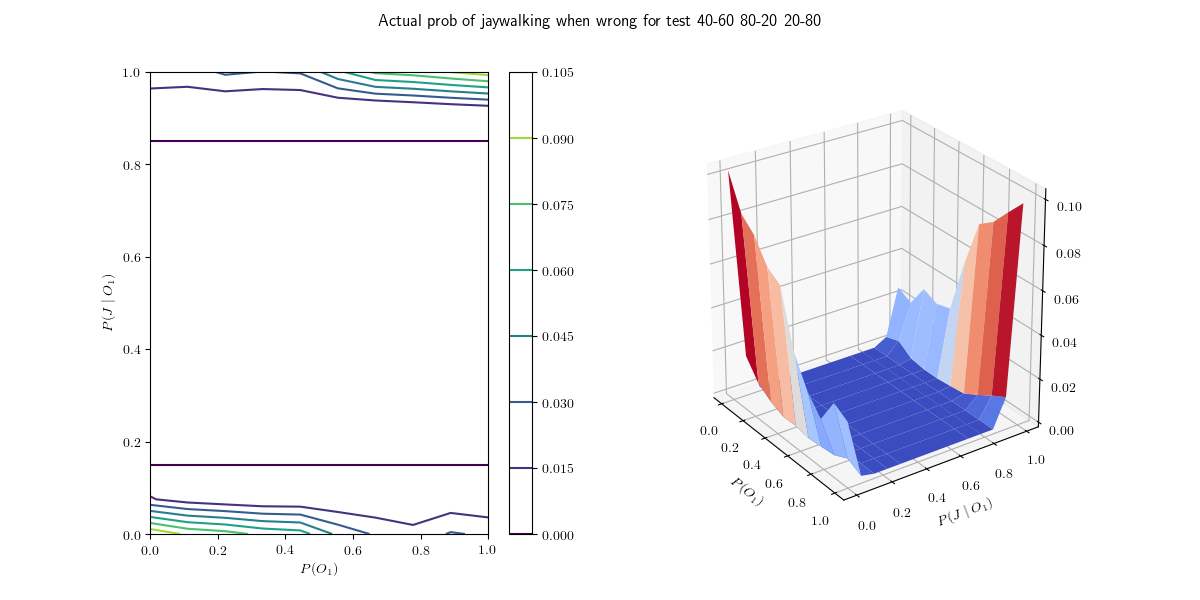
\includegraphics[scale=0.55]{test_40-60_80-20_20-80_jay_prob.png}}
    \caption[]{The actual jaywalking probability when classified incorrectly against \code{test 40-60 80-20 20-80}.}
    \label{fig:test_40-60_80-20_20-80_jay_prob_plot}
\end{figure}

% 
% test 40-60 20-80 80-20
% 

\begin{figure}[h]
    \centering
    \centerline{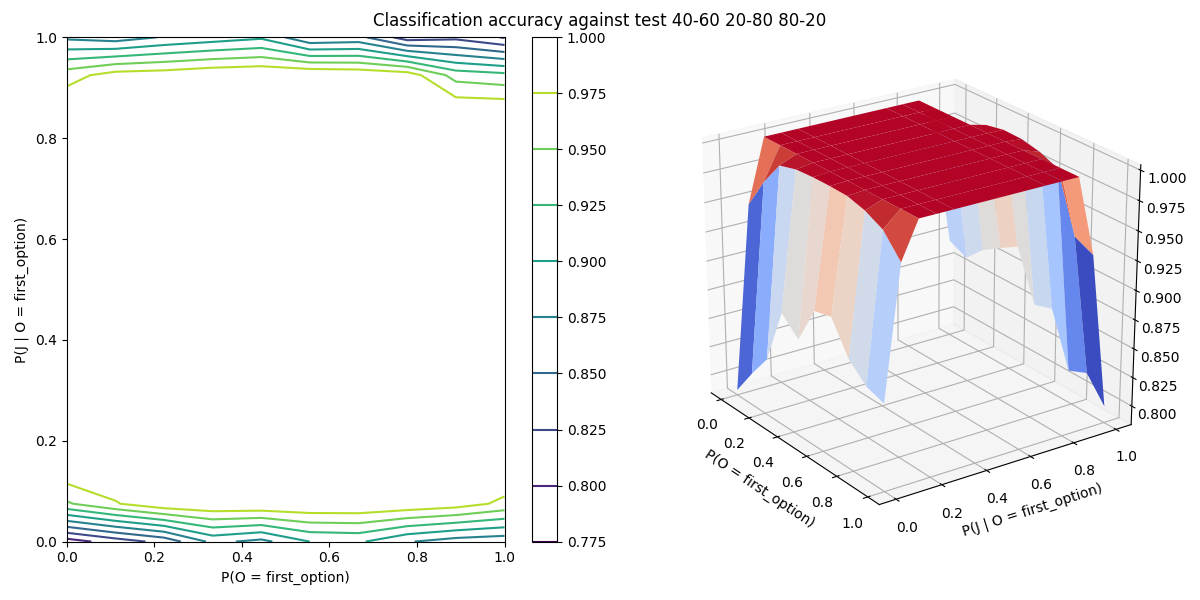
\includegraphics[scale=0.55]{test_40-60_20-80_80-20_accuracy.png}}
    \caption[]{The classification accuracy against \code{test 40-60 20-80 80-20}.}
    \label{fig:test_40-60_20-80_80-20_accuracy_plot}
\end{figure}

\begin{figure}[h]
    \centering
    \centerline{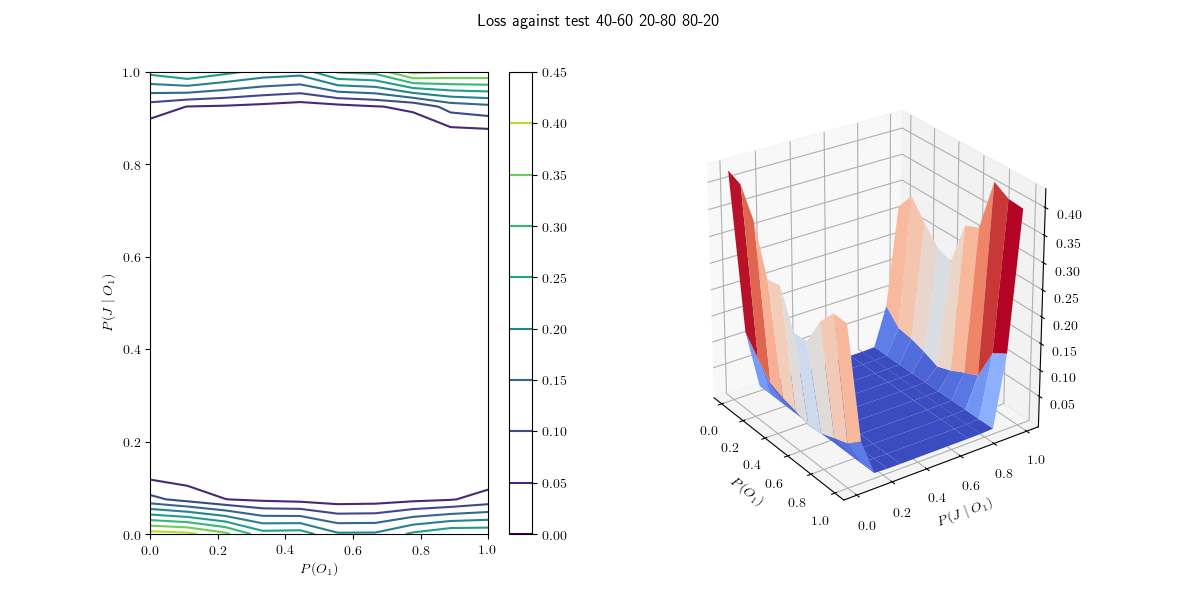
\includegraphics[scale=0.55]{test_40-60_20-80_80-20_loss.png}}
    \caption[]{The loss against \code{test 40-60 20-80 80-20}.}
    \label{fig:test_40-60_20-80_80-20_loss_plot}
\end{figure}

\begin{figure}[h]
    \centering
    \centerline{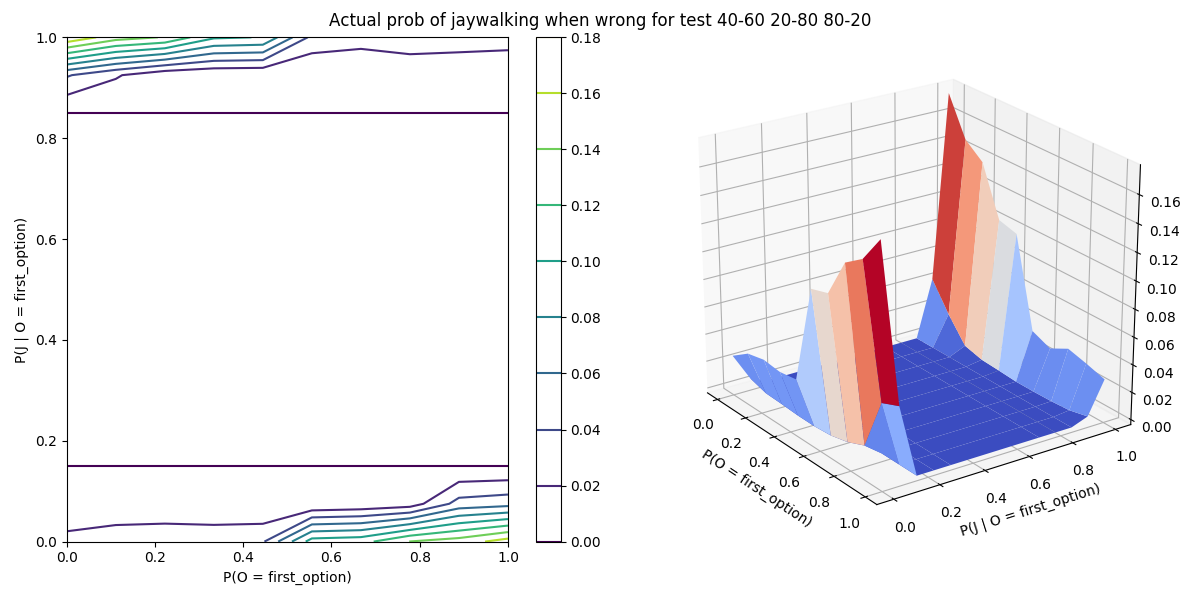
\includegraphics[scale=0.55]{test_40-60_20-80_80-20_jay_prob.png}}
    \caption[]{The actual jaywalking probability when classified incorrectly against \code{test 40-60 20-80 80-20}.}
    \label{fig:test_40-60_20-80_80-20_jay_prob_plot}
\end{figure}

% 
% test 50-50 50-50 50-50
% 

\begin{figure}[h]
    \centering
    \centerline{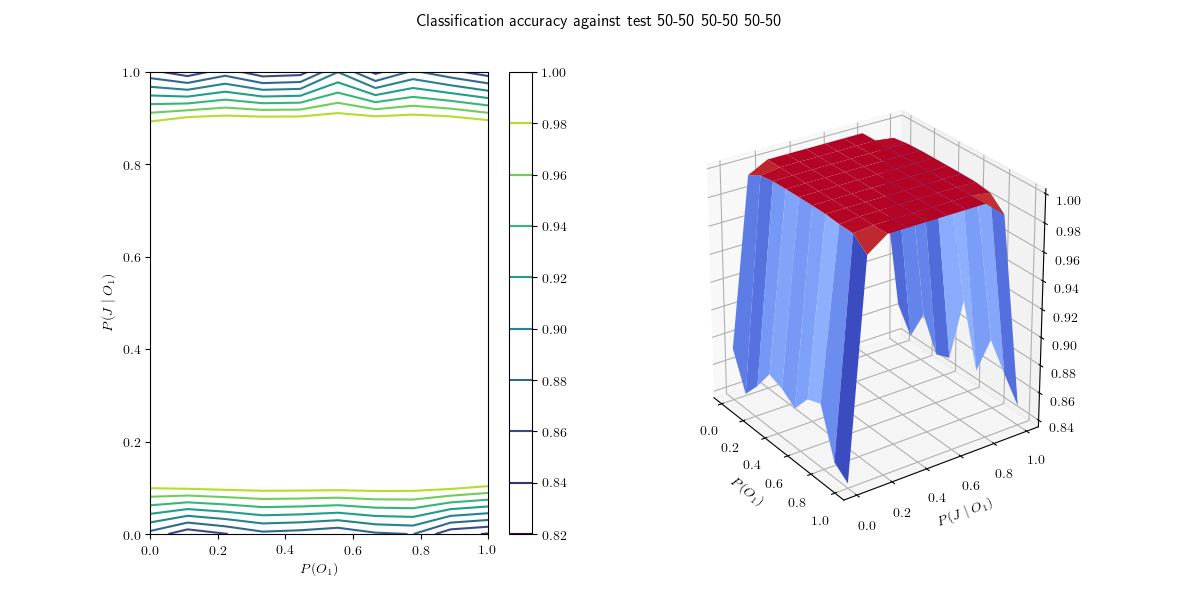
\includegraphics[scale=0.55]{test_50-50_50-50_50-50_accuracy.png}}
    \caption[]{The classification accuracy against \code{test 50-50 50-50 50-50}.}
    \label{fig:test_50-50_50-50_50-50_accuracy_plot}
\end{figure}

\begin{figure}[h]
    \centering
    \centerline{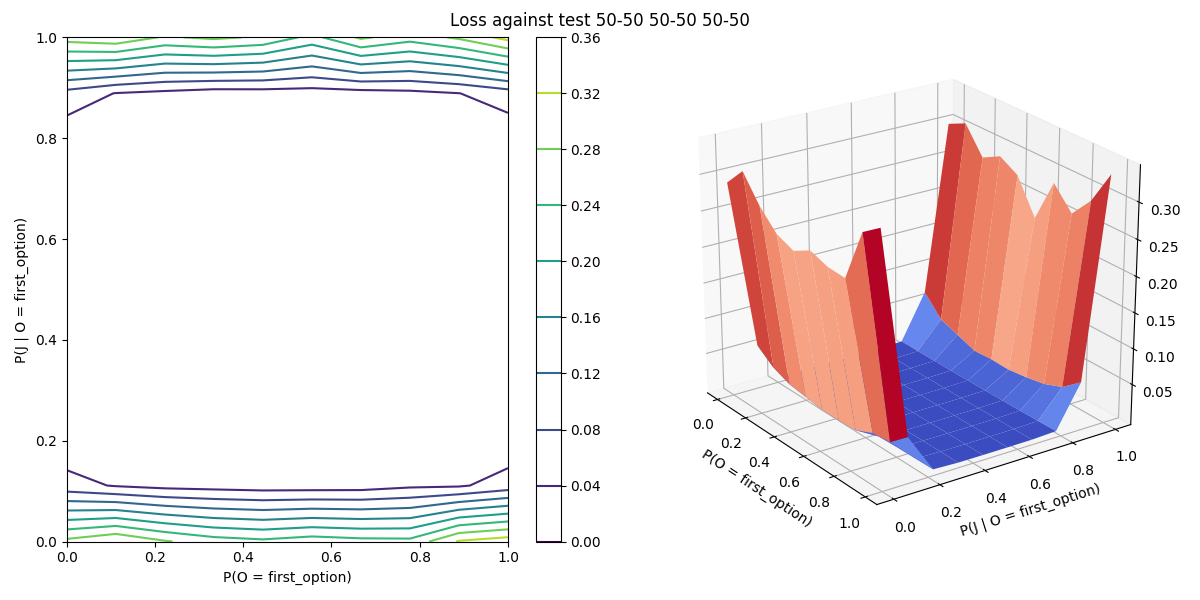
\includegraphics[scale=0.55]{test_50-50_50-50_50-50_loss.png}}
    \caption[]{The loss against \code{test 50-50 50-50 50-50}.}
    \label{fig:test_50-50_50-50_50-50_loss_plot}
\end{figure}

\begin{figure}[h]
    \centering
    \centerline{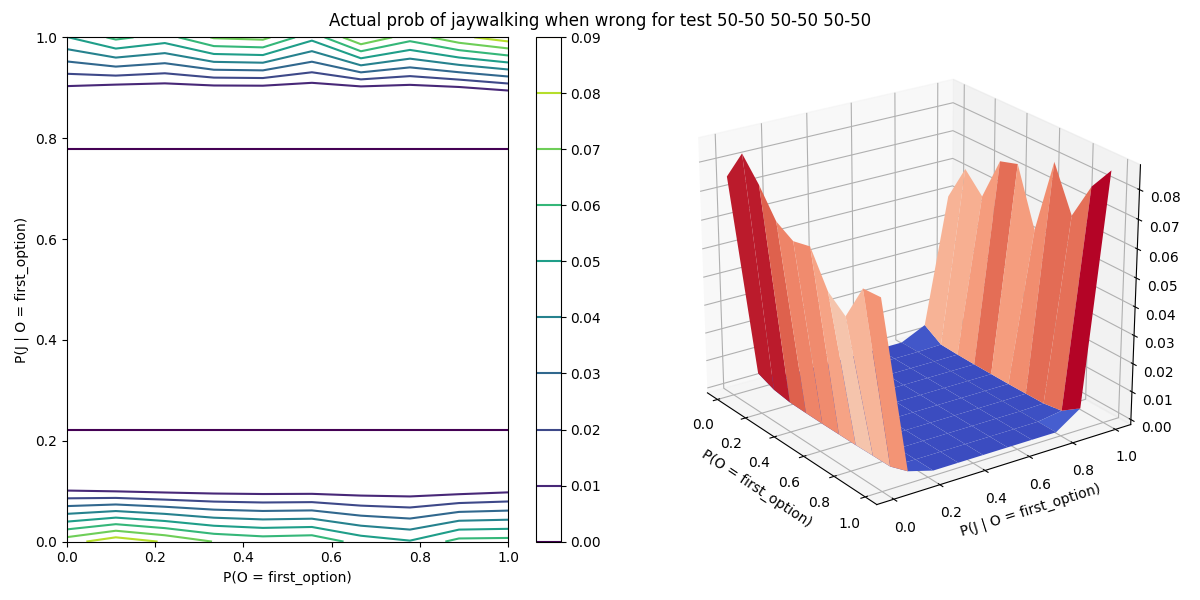
\includegraphics[scale=0.55]{test_50-50_50-50_50-50_jay_prob.png}}
    \caption[]{The actual jaywalking probability when classified incorrectly against \code{test 50-50 50-50 50-50}.}
    \label{fig:test_50-50_50-50_50-50_jay_prob_plot}
\end{figure}

\end{document}
